\subsection{pCVD Diamond Pad Detectors}
\begin{frame}{Setup}
	
	\begin{itemize}
		\itemfill
		\item rate studies conducted with \SI{260}{\mega\electronvolt\per c} $\uppi^+$ at Paul Scherrer Institute (PSI)
		\item tunable particle fluxes from \orderof{\SI{1}{\kilo\hertz\per cm^2}} to \orderof{\SI{10}{\mega\hertz\per cm^2}}
		\item detectors tested in ETHZ beam telescope (based on CMS-Pixel-Chips)
	\end{itemize}

	\vspace*{-5pt}
	\begin{figure}[h] 
		\centering
		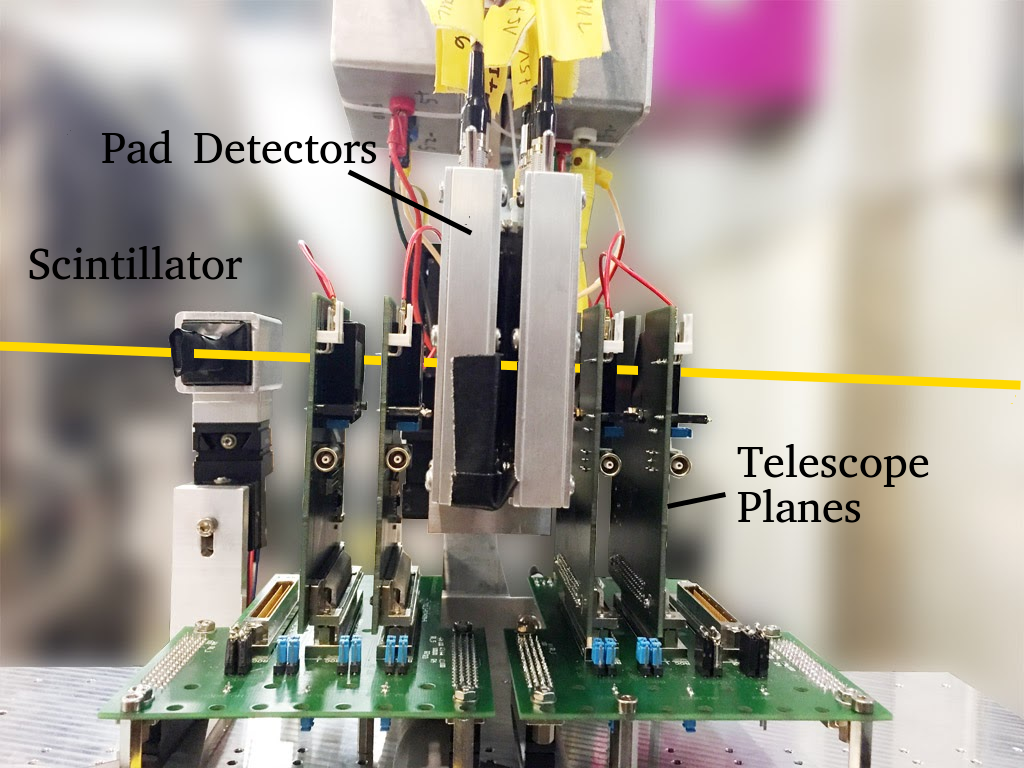
\includegraphics[height=.4\textheight]{Setup}
	\end{figure}
	\vspace*{-5pt}
	
	\begin{itemize}
		\item 4 tracking planes with particle trigger
		\item scintillator for precise trigger timing \ra \orderof{\SI{1}{\nano\second}}
	\end{itemize}

\end{frame}

% ============================ FRAME 2 ============================================
\begin{frame}{Pad Detectors}

	\begin{figure}[h] 
		\centering
		\begin{subfigure}{0.45\textwidth}  
			\centering
			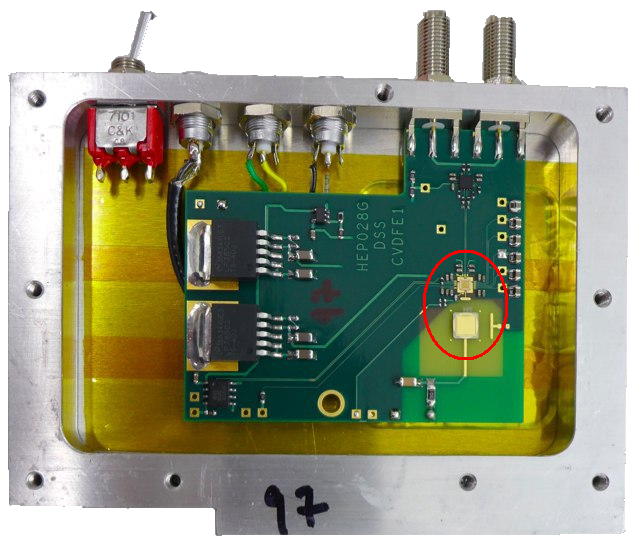
\includegraphics[height=0.45\textheight]{PadBox}
			\caption{fast amplifier box}
		\end{subfigure}
		\begin{subfigure}{0.45\textwidth} 
			\centering
			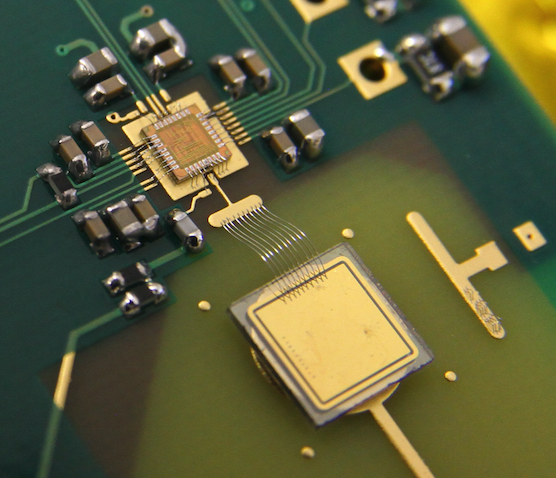
\includegraphics[height=0.45\textheight]{PadFull}
			\caption{diamond and fast amp} 	
		\end{subfigure} 
	\end{figure}
	\vspace*{-10pt}
	
	\begin{itemize}
		\itemfill
		\item diamonds in custom built amplifier boxes from Ohio State University (OSU)
		\item cleaning, photo-lithography and Cr-Au metallisation at OSU
		\item low noise, fast amplifier with \orderof{\z{5ns}} rise time
		\item prototype for HL-LHC BCM/BLM
	\end{itemize}
	
\end{frame}
% ============================ FRAME 3 ==========================================>
\begin{frame}{Waveforms}
	\vspace*{-20pt}
	\begin{center}
		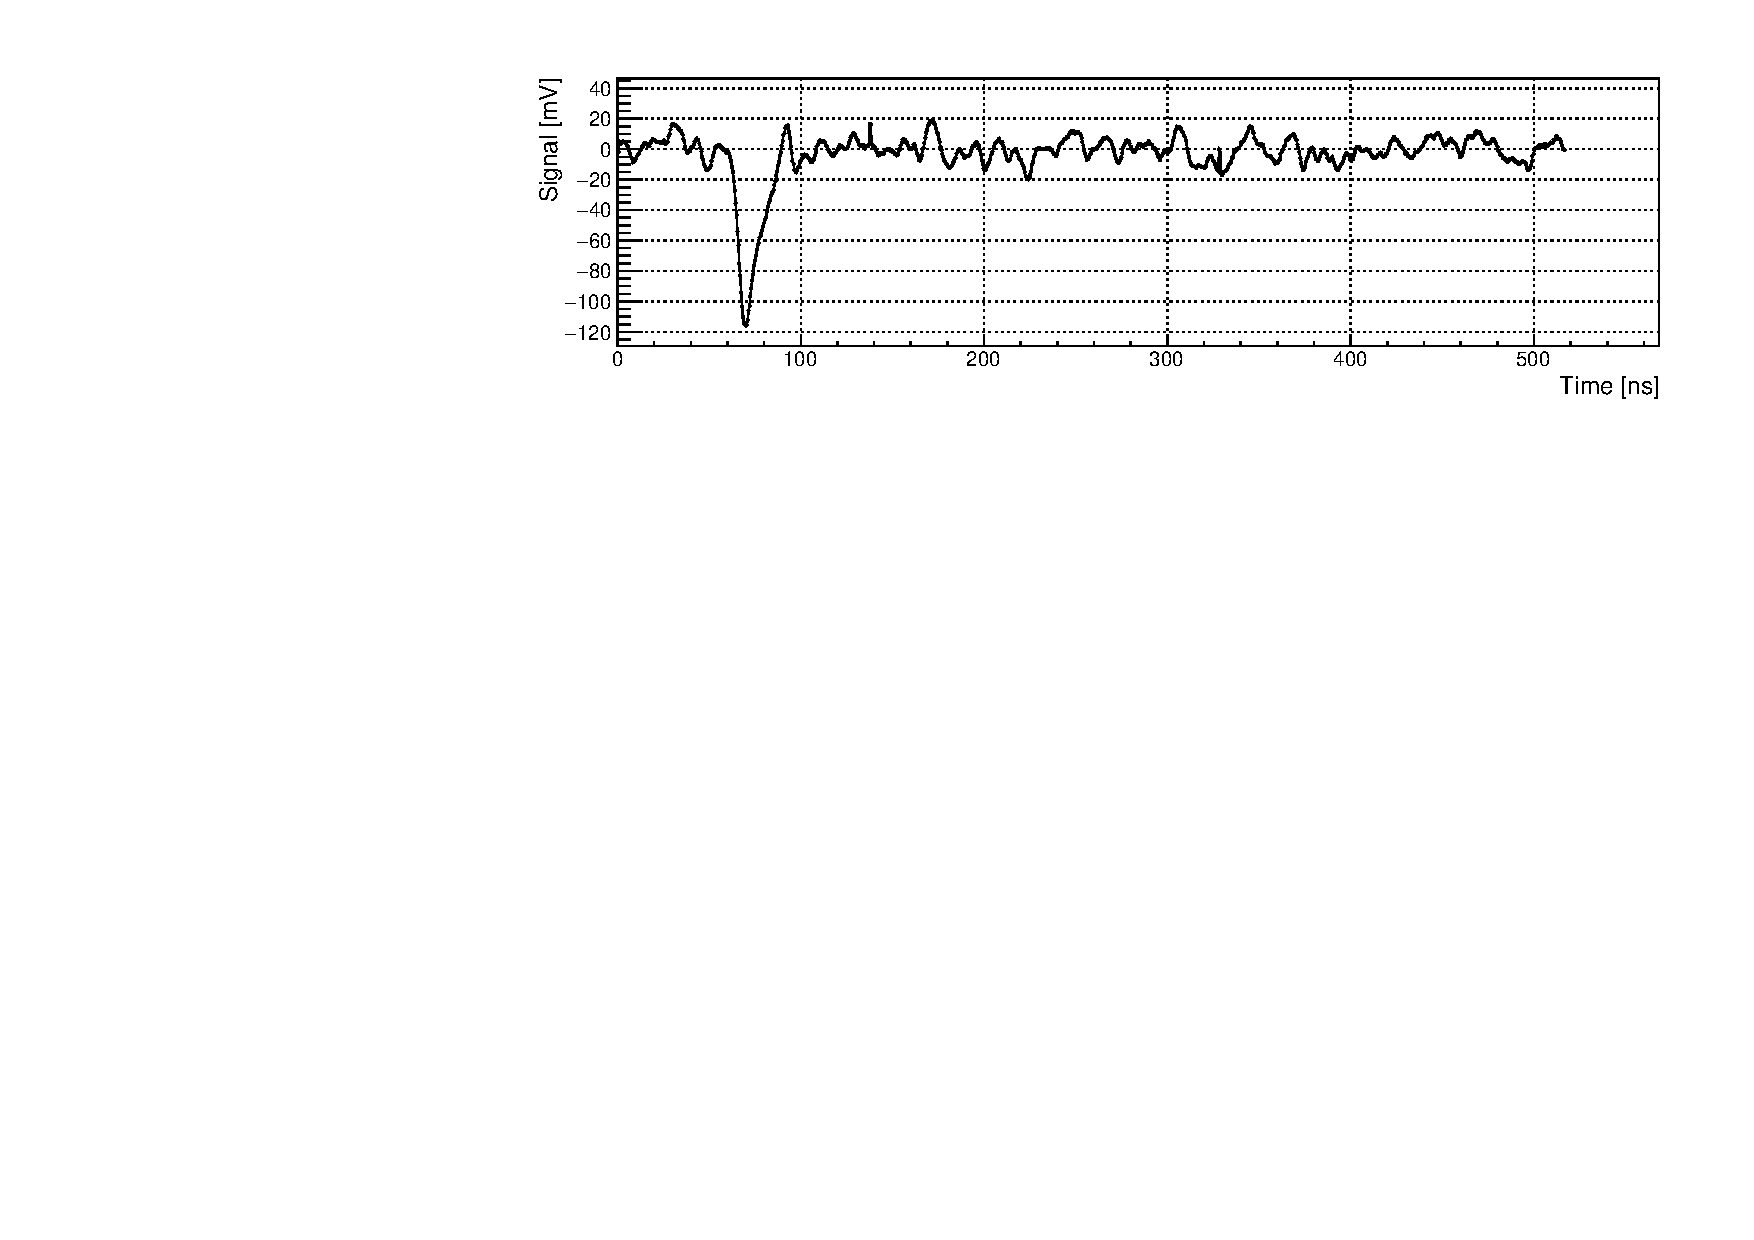
\includegraphics[angle=270, width=.73\textwidth]{SignalWaveform}\\
		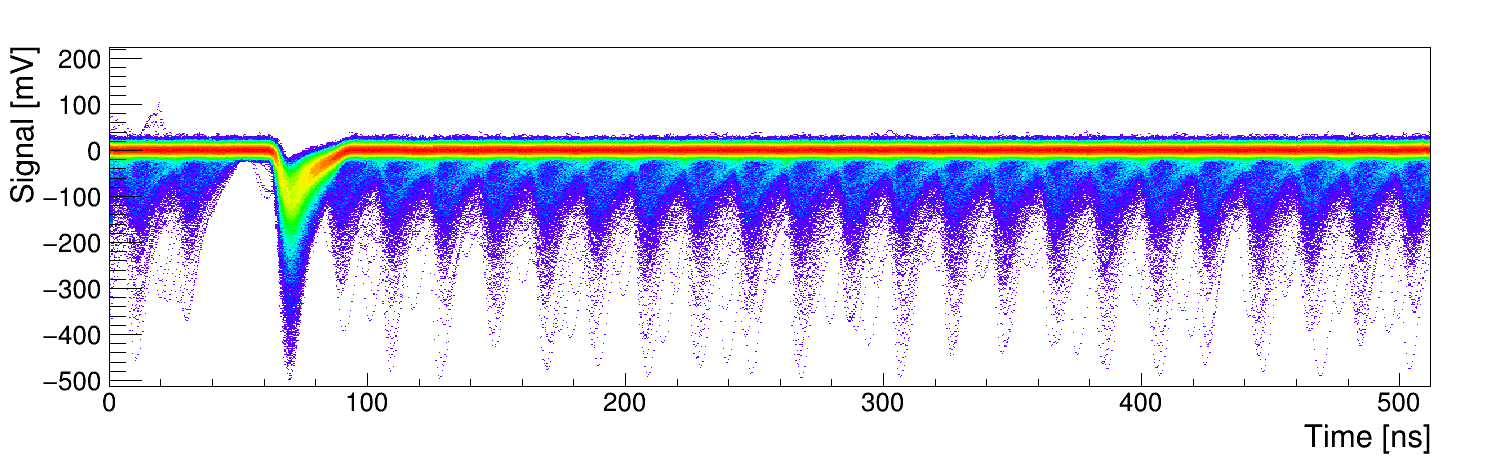
\includegraphics[width=.73\textwidth]{SignalWaveforms30000}
	\end{center}
	\begin{itemize}
		\item fast amplifier and good timing resolution \ra resolve bunch structure of PSI beam
		\item bunch spacing of \SI{19.8}{ns} clearly visible
	\end{itemize}
\end{frame}
% ============================ FRAME 4 ==========================================>
\begin{frame}{Results}

	\vspace*{-5pt}
	\begin{figure}[h]
		\begin{center}
			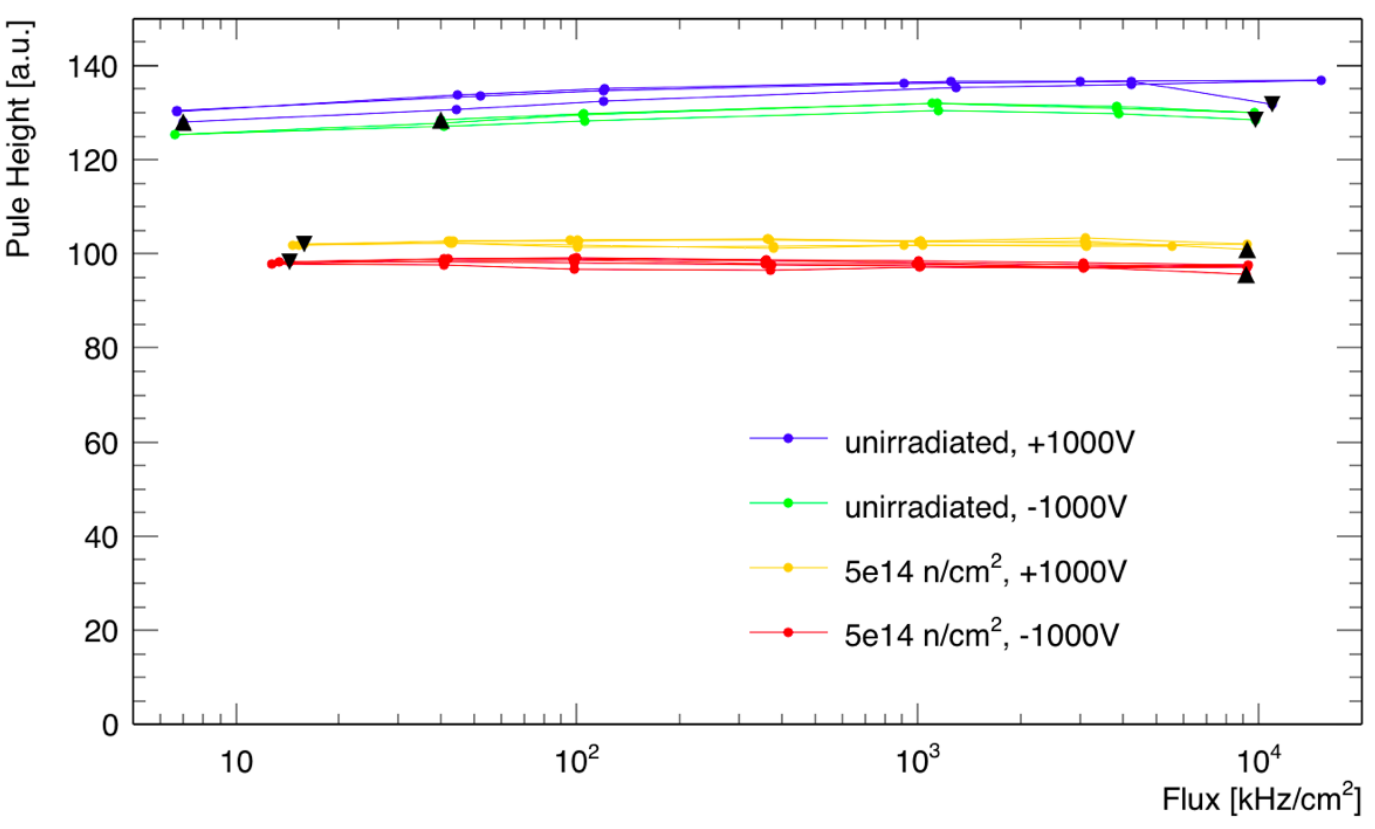
\includegraphics[width=.7\textwidth]{PadRates}
		\end{center}
	\end{figure}

	\begin{itemize}
		\item no rate dependence observed in pCVD diamonds up to \SI{10}{\mega\hertz\per cm^2}
		\item no absolute pulse height and noise calibration yet
		\item extending radiation doses to \SI{1e16}{n\per cm^2}
	\end{itemize}
\end{frame}
